% This is samplepaper.tex, a sample chapter demonstrating the
% LLNCS macro package for Springer Computer Science proceedings;
% Version 2.20 of 2017/10/04
%
\documentclass[runningheads]{llncs}

\usepackage{amsmath}
\usepackage{todonotes}

\usepackage[T1]{fontenc}
\usepackage{inconsolata}

% !TEX root = samplepaper.tex

% from https://tex.stackexchange.com/questions/173695/set-size-of-colorbox-for-a-single-character
\newcommand{\ColorBox}[2]{\colorbox{#1}{\makebox[\width]{\strut#2}}}
\setlength{\fboxsep}{0pt}

\usepackage{listingsutf8}
\lstdefinelanguage{hazel}{%
	morekeywords={let,in,case,end,.,|},
	sensitive=false,
	morecomment=[l]{--},
}
\usepackage{color}
\definecolor{comment}{RGB}{128,128,128}
\definecolor{stringColor}{RGB}{147,112,219}
\lstset{%
	language=hazel,
	numbers=left,
	numberstyle=\tiny\ttfamily,
	basicstyle=\small\ttfamily\linespread{0.8},
	tabsize=2,
	keywordstyle=\bfseries,
	commentstyle=\bfseries\color{comment},
	morestring=[d]{"},
	stringstyle=\color{stringColor},
	showstringspaces=false,
	mathescape,
	frame=trbl,
	rulecolor=\color{comment},
	escapeinside={@}{@},
	moredelim=[is][\ColorBox{red}]{/h/}{/h/},
}

\usepackage{bm}
\newcommand{\fnarrow}{$\bm{\rightarrow}$}
\newcommand{\lam}{$\bm{\lambda}$}
\newcommand{\casearrow}{$\bm{\Rightarrow}$}


\usepackage{tikz}

\usetikzlibrary{decorations.text}

\newcommand\myboxs[1]{\tikz[remember picture,overlay]\node(mk1){};}

\newcommand\myboxe[1]%
{
\tikz[remember picture,overlay]\node(mk2){};
\begin{tikzpicture}[remember picture,overlay]
\draw[green,dashed]([shift={(-2pt,1.5ex)}]mk1)rectangle([shift={(1pt,-0.5ex)}]mk2);
\end{tikzpicture}
}


\usepackage{xspace}
\newcommand{\Hazel}{\textsf{Hazel}\xspace}

%
\usepackage{graphicx}
% Used for displaying a sample figure. If possible, figure files should
% be included in EPS format.
%
% If you use the hyperref package, please uncomment the following line
% to display URLs in blue roman font according to Springer's eBook style:
% \renewcommand\UrlFont{\color{blue}\rmfamily}

% !TEX root = main.tex

\newcommand{\mynote}[3]{\textcolor{#3}{\textsf{{#2}}}}
\newcommand{\rkc}[1]{\mynote{rkc}{#1}{blue}}
\newcommand{\cy}[1]{\mynote{cy}{#1}{purple}}
\newcommand{\mah}[1]{\mynote{cy}{#1}{green}}
\newcommand{\matt}[1]{{\color{blue}{\textit{Matt:~#1}}}}

\newcommand{\cvert}{{\,{\vert}\,}}

%% https://tex.stackexchange.com/questions/9796/how-to-add-todo-notes
\newcommand{\rkcTodo}[1]{\todo[linecolor=blue,backgroundcolor=blue!25,bordercolor=blue]{#1}}

\newcommand{\mattTodo}[1]{\todo[linecolor=green,backgroundcolor=green!2,bordercolor=green]{\tiny\textit{#1}}}
\newcommand{\mattOmit}[1]{\colorbox{yellow}{(Matt omitted stuff here)}}

\def\parahead#1{\paragraph{\textbf{#1.}}}
%% \def\paraheadNoDot#1{\paragraph{{\textbf{#1}}}}
\def\subparahead#1{\paragraph{\textit{#1.}}}
%% \def\paraheadindent#1{\paragraph{}\textit{#1.}}
%% \def\paraheadindentnodot#1{\paragraph{}\textit{#1}}

% \newcommand{\ie}{{\emph{i.e.}}}
% \newcommand{\eg}{{\emph{e.g.}}}
% \newcommand{\etc}{{\emph{etc.}}}
% \newcommand{\cf}{{\emph{cf.}}}
% \newcommand{\etal}{{\emph{et al.}}}

%% \newcommand{\hazel}{\ensuremath{\textsc{Hazel}}}
%% \newcommand{\sns}{\ensuremath{\textsc{Sketch-n-Sketch}}}
%% \newcommand{\deuce}{\ensuremath{\textsc{Deuce}}}
\newcommand{\Elm}{\ensuremath{\textsf{Elm}}}
\newcommand{\sns}{\ensuremath{\textrm{Sketch-n-Sketch}}}
\newcommand{\deuce}{\ensuremath{\textrm{Deuce}}}

\newcommand{\sectionDescription}[1]{\section{#1}}
\newcommand{\subsectionDescription}[1]{\subsection{#1}}
\newcommand{\subsubsectionDescription}[1]{\subsubsection{#1}}
%% \newcommand{\subsectionDescription}[1]{\subsection*{#1}}
\newcommand{\suppMaterials}{the Supplementary Materials}

\newcommand{\defeq}{\overset{\textrm{def}}{=}}

\newcommand{\eap}{action suggestion panel\xspace}
\newcommand{\Eap}{Action suggestion panel\xspace}

\newcommand{\myfootnote}[1]{\footnote{ #1}}

\def\sectionautorefname{Section}
\def\subsectionautorefname{Section}
\def\subsubsectionautorefname{Section}

\newcommand{\code}[1]{\lstinline{#1}}

% Make italic?
%\newcommand{\Property}[1]{\emph{#1}}
\newcommand{\Property}[1]{\textrm{#1}}

% Calling out Cyrus's favorite verb, 'to be' ;)
\newcommand{\IS}{\colorbox{red}{is}\xspace}

\newcommand{\codeSize}
  %% {\footnotesize}
  {\small}

%\newcommand{\JoinTypes}[2]{\textsf{join}~~#1~~#2}
\newcommand{\JoinTypes}[2]{\textsf{join}(#1,#2)}

%%%%%%%%%%%%%%%%%%%%%%%%%%%%%%%%%%%%%%%%%%%%%%%%%%%%%%%%%%%%%%%%%%%%%%%%%%%%%%%%
%% Spacing

\newcommand{\sep}{\hspace{0.06in}}
\newcommand{\sepPremise}{\hspace{0.20in}}
\newcommand{\hsepRule}{\hspace{0.20in}}
\newcommand{\vsepRuleHeight}{0.08in}
\newcommand{\vsepRule}{\vspace{\vsepRuleHeight}}
\newcommand{\miniSepOne}{\hspace{0.01in}}
\newcommand{\miniSepTwo}{\hspace{0.02in}}
\newcommand{\miniSepThree}{\hspace{0.03in}}
\newcommand{\miniSepFour}{\hspace{0.04in}}
\newcommand{\miniSepFive}{\hspace{0.05in}}

%%%%%%%%%%%%%%%%%%%%%%%%%%%%%%%%%%%%%%%%%%%%%%%%%%%%%%%%%%%%%%%%%%%%%%%%%%%%%%%%

% \lstset{
% %mathescape=true,basicstyle=\fontsize{8}{9}\ttfamily,
% literate={=>}{$\Rightarrow$}2
%          {<=}{$\leq$}2
%          {->}{${\rightarrow}$}1
%          {\\\\=}{\color{red}{$\lambda$}}2
%          {\\\\}{$\lambda$}2
%          {**}{$\times$}2
%          {*.}{${\color{blue}{\texttt{*.}}}$}2
%          {+.}{${\color{blue}{\texttt{+.}}}$}2
%          {<}{${\color{green}{\lhd}}$}1
%          {>?}{${\color{green}{\rhd}}$?}2
%          {<<}{${\color{green}{\blacktriangleleft}}$}1
%          {>>?}{${\color{green}{\blacktriangleright}}$?}2
%          {\{}{${\color{blue}{\{}}$}1
%          {\}}{${\color{blue}{\}}}$}1
%          {[}{${\color{purple}{[}}$}1
%          {]}{${\color{purple}{]}}$}1
%          {(}{${\color{darkgray}{\texttt{(}}}$}1
%          {)}{${\color{darkgray}{\texttt{)}}}$}1
%          {]]}{${\color{gray}{\big(}}$}1
%          {]]}{${\color{gray}{\big)}}$}1
% }


\begin{document}
%
\title{Flexible Structure Editing via Node Staging}
%
%\titlerunning{Abbreviated paper title}
% If the paper title is too long for the running head, you can set
% an abbreviated paper title here
%
\author{David Moon\inst{1} \and
Cyrus Omar\inst{2} \and
R.~Benjamin Shapiro\inst{1}}
%
\authorrunning{David Moon, Cyrus Omar, and R.~Benjamin Shapiro}
% First names are abbreviated in the running head.
% If there are more than two authors, 'et al.' is used.
%
\institute{University of Colorado Boulder, Boulder CO 80309, USA\and
University of Chicago, Chicago IL 60637, USA}
%Springer Heidelberg, Tiergartenstr. 17, 69121 Heidelberg, Germany
%\email{lncs@springer.com}\\
%\url{http://www.springer.com/gp/computer-science/lncs} \and
%ABC Institute, Rupert-Karls-University Heidelberg, Heidelberg, Germany\\
%\email{\{abc,lncs\}@uni-heidelberg.de}}
%
\maketitle              % typeset the header of the contribution
%
\begin{abstract}
Structure editors allow programmers to edit the tree structure of a program directly.
They can provide cognitive benefits for novice programmers, simplify language composition, 
and improve the availability of editor services. They are also known for being hard 
to use.

We present the structure editor design of \Hazel, a live functional programming
environment. \Hazel's type-aware edit actions and execution semantics for incomplete programs ensure that every reachable edit state is not only syntactically well-formed, but also statically and dynamically well-defined. This unique invariant of \Hazel adds new motivation to improve the ergonomics of structure editing. 

In our effort to do so, we incorporate a novel \emph{node staging} mode to resolve ambiguous user intent when wrapping and unwrapping parent nodes around their children. Just as code completion menus facilitate exploration of valid token completions, node staging facilitates exploration of valid placements of a node's syntactic delimiters. It also makes it easy to preserve children nodes when removing their parent. We motivate and describe our design choices, compare our design to prior work, and describe our plan for user evaluation.
%key points
%\begin{itemize}
%\item in progress of scaling up usability of core Hazelnut calculus
%\item structure editing eliminates syntax errors, in Hazel enables live computation
%\item we propose a design that marries affordances of linear text and structure trees
%\end{itemize}
%\keywords{First keyword  \and Second keyword \and Another keyword.}
\end{abstract}
%
%
%
\section{Introduction}
Plain text dominates as the universal format for computer programs. Although the simplicity and generality of text are extremely useful, the benefits come at 
some costs. For novice programmers, the 
unrestricted nature of text leaves room for syntax errors that make learning how to program 
more difficult \cite{text_vs_frame}. Plain text also
complicates the design of language-aware editor services. Because many sequences of 
characters do not correspond to meaningful programs, these services flicker in and out of 
availability, or their implementations must deploy \emph{ad hoc} heuristics, e.g., by using 
whitespace to guess intent 
\cite{error_recovery_generated_parser,rapid_feedback_generated_parser}.

These issues have motivated a long line of research into \emph{structure editors}, i.e., 
program editors where every edit state corresponds to a program structure \cite{cornell}.
Structure editors limit unstructured text editing to within well-formed structures and 
otherwise rely on operations that create and manipulate structural components.
In so doing, they avoid classes of syntax errors that may otherwise arise in plain text. This 
has proven useful for teaching children how to program, as demonstrated by the popularity of 
the structure editor Scratch \cite{scratch}. 

Recent work shows structure editing can support additional powerful advantages. The Jetbrains MPS language workbench uses a structure editor to enable clean composition of domain-specific languages as well as end-user-friendly graphical notations \cite{lessons_learned_mps}. Meanwhile, the functional programming language and environment \Hazel uses structure editing to enforce \emph{semantic} validity. Uniquely, \Hazel's type-aware edit actions and execution semantics for incomplete programs ensure that every reachable edit state is not only syntactically well-formed, but also statically and dynamically well-defined \cite{hazelnut,hazelnut_live}.

Despite all these advantages, structure editors have not achieved widespread adoption. They do not integrate well with existing toolchains built for the plain text format \cite{towards_user_friendly_projectional_editors}, and they are known for usability issues such as being hard to learn \cite{towards_user_friendly_projectional_editors,efficiency_of_projectional_editing} and scaling poorly to large programs \cite{blocks_at_your_fingertips}. In this paper, we focus our attention on the latter problem of usability.

We present the structure editor design of \Hazel. Our design improves on prior work by incorporating a novel \emph{node staging} mode that resolves ambiguous user intent when wrapping and unwrapping parent nodes around their children. 

\parahead{Paper Outline} We begin in Sec.~\ref{sec:related-work} by reviewing prior work on improving the usability of structure editors. This review motivates our design principles, which we state in Sec.~\ref{sec:design} followed by an example-driven overview of \Hazel's structure editor. Sec.~\ref{sec:conclusion} describes future work and concludes.

\section{Related Work} \label{sec:related-work}
\begin{itemize}
	\item prior work on improving usability for inputting sequences of infix operators
  	\begin{itemize}
  		\item early structure editors like Cornell Synthesizer \cite{cornell} stepped around issue of infix operator sequences by resorting to text editing at leaves
  		\item other editors leverage a form of online precedence parsing to restructure the tree as needed
  	\end{itemize}
	\item comparatively, little innovation on interface for complex node construction and removal, that is, creating a new node that wraps around existing code, and removing a node while preserving or moving its children
		\begin{itemize}
			\item we believe interface for such operations in today's structure editors is key contributor to users' negative perceptions of structure editing
		\end{itemize}
	\item in a controlled experiment comparing user efficiency for MPS vs a text editor \cite{efficiency_of_projectional_editing}, Berger et al.~observe that novice users of structure editors perceive selection as inaccurate compared to other operations, and that \emph{both} novice and proficient users of structure editors perceive deletion as inaccurate compared to other operations.
		\begin{itemize}
			\item responses to a post-survey questionnaire reveal that structure editor users felt that they often deleted more than they expected, motivating our desire for a better interface for complex deletions
		\end{itemize}
	\item meanwhile, selection is essential for node construction in existing structure editors
		\begin{itemize}
			\item either the user must select a child node before applying a construction operation or the user must create the node and then select and move existing nodes into it
			\item thus, usability issues for selection affect node construction as well
		\end{itemize}
	\item additionally, we conjecture that node construction is awkward for novice users of structure editors because it inverts the usual order of operations when constructing nodes in text editors
%		\begin{itemize}
%			\item yada yada \todo{coalesce this paragraph with previous paragraph}
%		\end{itemize}
\end{itemize}


%\begin{itemize}
%\item A comparative study of moded and modeless text editing by experienced editor users by Poller \& Garter \url{https://dl.acm.org/citation.cfm?id=801603}
%\item A personal history of modeless text editing and cut/copy-paste by Tesler \url{https://dl.acm.org/citation.cfm?id=2212896}
%\item The Smalltalk Environment by Tesler \url{https://tech-insider.org/star/research/acrobat/8108-a.pdf}
%\item Modeling Human-Machine Systems: On Modes, Error, and Patterns of Interaction by Degani % https://ti.arc.nasa.gov/m/profile/adegani/Degani_Thesis.pdf
%\item Modes in User Interfaces: When They Help and When They Hurt Users \url{https://www.nngroup.com/articles/modes/}
%\item The keystroke-level model for user performance time with interactive systems by Card et al. \url{https://dl.acm.org/citation.cfm?doid=358886.358895}
%\item ParEdit \url{https://www.emacswiki.org/emacs/ParEdit}
%\end{itemize}


\section{Design} \label{sec:design}

\subsection{Principles}

(WIP list)
\begin{itemize}
\item Users should be able to hold Backspace/Delete to delete everything before/after the cursor.
\item Users should be able to perform arbitrary deletions.
\item Deletions should be clearly indicated before they happen.
\item Users should be able to choose the node to construct before choosing its children.
\item Users should never have to follow two moving parts.
\end{itemize}

guided by overall text like experience, you want to operate on a tree like structure but enable linear operations as suggested by the layout, doesn't preclude tree operations or tree affordances/signifiers
\begin{itemize}
\item text-like cursor, single point of focus, differs from POPL 17 paper
\item deletion
\item operator sequences
\item selection model + cut/copy
\item line items (linearing tree)
\item keywords
\item tabbing between holes
\item cursor inspector, what is highlighted under the cursor, what is the mapping between text cursor and semantic cursor
\item transitory edit mode
\item shifting parentheses/delimiters (mark shift points, highlight points with least errors (maybe a single highlighted suggestion to minimize clutter)?)
\item maybe swapping
\item maybe mention inlining context inspector, put live values in side of code
\end{itemize}




\subsection{Example}

We now provide an example-driven overview of \Hazel's editing mechanics.
We walk through how one might implement in \Hazel the function \texttt{str\_of\_list},
which takes a list of numbers and returns its string representation. We
elide most steps and focus on a few interesting edit transitions. We refer
back to our design principles as they are demonstrated concretely.

In the rest of this section, each consecutive pair of programs connected
visually by a line represents a single edit transition. Text between the
start and end state of each edit describes the edit and relevant features of
\Hazel. Elided steps are denoted by ellipses between pairs of programs.
%\todo{add mention of cursor inspector, other editor services we are omitting
%to focus on editing mechanics}

\noindent
\begin{hazel}
<h>_</h>
\end{hazel}
	\begin{tabular}{|p{\linewidth}}
	We begin with an empty expression hole.
	\textcolor{red}{(Add something here about expression holes.)}
	\textcolor{red}{(Also something about the text-like cursor.)}
	We would first like to define a variable \texttt{str\_of\_list}, so we begin typing out the keyword
	\texttt{let}. 
	\end{tabular}
\begin{hazel}
<c>le</c>
\end{hazel}
	\begin{tabular}{|p{\linewidth}}
	As we type, the editor identifies \texttt{le} as an unbound variable and indicates this
	fact with an orange dotted border.
	\end{tabular}
\begin{hazel}
<c>let</c>
\end{hazel}
	\begin{tabular}{|p{\linewidth}}
	Upon typing out the reserved keyword \texttt{let}, indicated by the bold font, we invoke
	construction of a let line by hitting Space.
	\end{tabular}
\begin{hazel}
let <c>_</c> = <h>_</h> in
<h>_</h>
\end{hazel}
	\[\vdots\]
\begin{hazel}
let <c>str_of_lst</c> = <h>_</h> in
<h>_</h>
\end{hazel}
	\begin{tabular}{|p{\linewidth}}
	Upon typing out the function name, we hit the Tab key to move our cursor to the next empty hole.
	\end{tabular}
\begin{hazel}
let str_of_lst = <c>_</c> in
<h>_</h>
\end{hazel}
	\begin{tabular}{|p{\linewidth}}
	We use Backslash to create a lambda expression.
	\end{tabular}
\begin{hazel}
let str_of_lst = @\lam @<c>_</c>.{<h>_</h>} in
<h>_</h>
\end{hazel}
	\[\vdots\]
\begin{hazel}
let str_of_lst = @\lam @ns.{<c>case</c>} in
<h>_</h>
\end{hazel}
	\begin{tabular}{|p{\linewidth}}
	Like \texttt{let}, \texttt{case} is a reserved keyword and can be used to construct
	a case expression by hitting Space after typing out the word.
	\end{tabular}
\begin{hazel}
let str_of_lst = 
	@\lam @ns.{
		case <c>_</c>
		| <h>_</h> @\casearrow @ <h>_</h>
		end
	}
in
<h>_</h>
\end{hazel}
	\[\vdots\]
\begin{hazel}
let str_of_lst = 
	@\lam @ns.{
		case ns
		| [] @\casearrow @ <c>""</c>
		end
	}
in
<h>_</h>
\end{hazel}
	\begin{tabular}{|p{\linewidth}}
	Pressing Enter at the end of a \texttt{case} rule creates a new rule.
	\end{tabular}
\begin{hazel}
let str_of_lst = 
	@\lam @ns.{
		case ns
		| [] @\casearrow @ ""
		| <c>_</c>  @\casearrow @ <h>_</h>
		end
	}
in
<h>_</h>
\end{hazel}
	\[\vdots\]
\begin{hazel}
let str_of_lst = 
	@\lam @ns.{
		case ns
		| []      @\casearrow @ ""
		| n :: [] @\casearrow @ <c>str_of_int</c>
		end
	}
in
<h>_</h>
\end{hazel}
	\begin{tabular}{|p{\linewidth}}
	Suppose we have the function \texttt{str\_of\_int} in scope.
	As we fill out the second rule, we encounter a type inconsistency,
	denoted by the red dotted border around \texttt{str\_of\_int} on
	Line 5. \Hazel expects the rule to have a return type of \texttt{String}
	but it has found a value of type \texttt{Num \fnarrow~String} instead.
	The type inconsistency is resolved once we hit Space to construct
	a function application.
	\end{tabular}
\begin{hazel}
let str_of_lst = 
	@\lam @ns.{
		case ns
		| []      @\casearrow @ ""
		| n :: [] @\casearrow @ str_of_int <c>_</c>
		end
	}
in
<h>_</h>
\end{hazel}
	\[\vdots\]
\begin{hazel}
let str_of_lst = 
	@\lam @ns.{
		case ns
		| []      @\casearrow @ ""
		| n :: [] @\casearrow @ str_of_int n		
		| n :: ns @\casearrow @ str_of_int n ++ "," ++ str_of_lst ns
		end
	}
in
<c>_</c>
\end{hazel}
	\begin{tabular}{|p{\linewidth}}
	At this point, we realize that we would like bookend the return string
	with brackets. This requires refactoring the current body of
	\texttt{str\_of\_lst} into its own internal recursive helper function.
	We add a new line above the \texttt{case} expression and create a
	\texttt{let} line.
	\end{tabular}
\begin{hazel}
let str_of_lst = 
	@\lam @ns.{
		let <h>_</h> = <h>_</h> [in]
		case ns
		| []      @\casearrow @ ""
		| n :: [] @\casearrow @ str_of_int n		
		| n :: ns @\casearrow @ str_of_int n ++ "," ++ str_of_lst ns
		end
	}
in
_
\end{hazel}
	\begin{tabular}{|p{\linewidth}}
	We have triggered \emph{node staging} mode. \Hazel has detected
	ambiguity in our intent: should the \texttt{case} expression be part of
	the defining expression of the \texttt{let} line we just constructed,
	or should it remain in the subsequent body expression? Such ambiguities
	can be reduced to ambiguity in where to place a syntactic delimiter
	of the node being constructed. In this case, the delimiter in question is
	\texttt{in} on Line 3. In node staging mode, the left and right
	keys cycle through viable placements of the delimiter in question.
	We want the \texttt{case} expression to be in the defining expression,
	i.e., we want the \texttt{in} delimiter to come after the \texttt{case}
	expression, so we press right to see the next viable position.
	\end{tabular}
\begin{hazel}
let str_of_lst = 
	@\lam @ns.{
		let <h>_</h> =
			case ns
			| []      @\casearrow @ ""
			| n :: [] @\casearrow @ str_of_int n		
			| n :: ns @\casearrow @ str_of_int n ++ "," ++ str_of_lst ns
			end
		[in]
		<h>_</h>
	}
in
_
\end{hazel}
	\begin{tabular}{|p{\linewidth}}
	The \texttt{case} expression has filled the empty hole previously in 
	the defining expression, and a new empty hole has been generated as the
	new body expression on Line 10.
	\end{tabular}
\begin{hazel}
let str_of_lst = 
	@\lam @ns.{
		let <h>_</h> =
			case ns
			| []      @\casearrow @ ""
			| n :: [] @\casearrow @ str_of_int n		
			| n :: ns @\casearrow @ str_of_int n ++ "," ++ str_of_lst ns
			end
		[in]
		<h>_</h>
	}
in
_
\end{hazel}
	\begin{tabular}{|p{\linewidth}}
	This is the position we want, so we press Enter to return to
	the usual editing mode.
	\end{tabular}
\begin{hazel}
let str_of_lst = 
	@\lam @ns.{
		let <h>_</h> =
			case ns
			| []      @\casearrow @ ""
			| n :: [] @\casearrow @ str_of_int n		
			| n :: ns @\casearrow @ str_of_int n ++ "," ++ str_of_lst ns
			end
		|in
		<h>_</h>
	}
in
_
\end{hazel}

\begin{hazel}
let str_of_lst =
	@\lam @ns.{
		let str_of_elems = 
			@\lam @ns.{
				case ns
				| []      @\casearrow @ ""                                     
				| n :: [] @\casearrow @ str_of_int n                           
				| n :: ns @\casearrow @ str_of_int n ++ "," ++ str_of_elems ns 
				end
			}
		in
		"[" ++ str_of_elems ns ++ "]"
	}
in
<h>_</h>
\end{hazel}


%\begin{figure}
%\begin{lstlisting}
%type Tm         -- term
%type Op         -- operator
%type Seq =      -- sequence of infix operators
%| TmOpTm Tm Op Tm
%| SeqOpTm OpSeq Op Tm
%	
%type SeqSurround =                  -- Seq zipper context
%| EmptyPrefix SeqSuffix             --  _ + tm + tm + ...
%| EmptySuffix SeqPrefix             --  ... + tm + tm + _
%| BothNonEmpty SeqPrefix SeqSuffix  --  ... + tm + _ + tm + ...
%and SeqPrefix =
%| TmPrefix Tm Op
%| SeqPrefix Seq Op
%and SeqSuffix =
%| TmSuffix Op Tm
%| SeqSuffix Op Seq
%\end{lstlisting}
%\end{figure}
%
%\begin{minipage}{\linewidth}
%\begin{lstlisting}
%let next_tm : (Tm, SeqSurround) @\fnarrow @ (Tm, SeqSurround) =
%	@\lam @(curr_tm, curr_surround).
%		case surround
%		| EmptySuffix prefix @\casearrow @
%			-- reader, look here --
%			let ( new_tm, new_suffix ) =
%				case prefix
%				| TmPrefix new_tm op @\casearrow @
%					let new_suffix = TmSuffix op curr_tm in
%					( new_tm, new_suffix )
%				| SeqPrefix seq op =>
%					let ( new_z, suffix ) = place_cursor_seq seq in
%					let new_suffix =
%						append_tm_to_suffix suffix op (erase z)
%					in
%					( new_tm, new_suffix )
%				end
%			in
%			@\myboxs{}@( new_z, EmptyPrefix new_suffix )@\myboxe{}@
%		end
%in
%_
%\end{lstlisting}
%\end{minipage}

\section{Conclusion} \label{sec:conclusion}

This summer, we will finish our implementation and evaluate our design via a user study.
We plan on recruiting participants from the Recurse Center, a self-directed educational retreat for programmers in New York City. We plan on having users walk through a variety of implementation and refactoring exercises within \Hazel, then qualitatively analyzing their edit logs and subjective responses.

%\newpage
%\subsection{A Subsection Sample}
%Please note that the first paragraph of a section or subsection is
%not indented. The first paragraph that follows a table, figure,
%equation etc. does not need an indent, either.
%
%Subsequent paragraphs, however, are indented.
%
%\subsubsection{Sample Heading (Third Level)} Only two levels of
%headings should be numbered. Lower level headings remain unnumbered;
%they are formatted as run-in headings.
%
%\paragraph{Sample Heading (Fourth Level)}
%The contribution should contain no more than four levels of
%headings. Table~\ref{tab1} gives a summary of all heading levels.
%
%\begin{table}
%\caption{Table captions should be placed above the
%tables.}\label{tab1}
%\begin{tabular}{|l|l|l|}
%\hline
%Heading level &  Example & Font size and style\\
%\hline
%Title (centered) &  {\Large\bfseries Lecture Notes} & 14 point, bold\\
%1st-level heading &  {\large\bfseries 1 Introduction} & 12 point, bold\\
%2nd-level heading & {\bfseries 2.1 Printing Area} & 10 point, bold\\
%3rd-level heading & {\bfseries Run-in Heading in Bold.} Text follows & 10 point, bold\\
%4th-level heading & {\itshape Lowest Level Heading.} Text follows & 10 point, italic\\
%\hline
%\end{tabular}
%\end{table}
%
%
%\noindent Displayed equations are centered and set on a separate
%line.
%\begin{equation}
%x + y = z
%\end{equation}
%Please try to avoid rasterized images for line-art diagrams and
%schemas. Whenever possible, use vector graphics instead (see
%Fig.~\ref{fig1}).
%
%\begin{figure}
%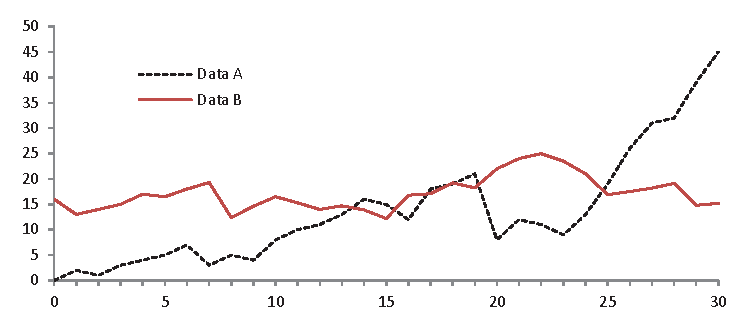
\includegraphics[width=\textwidth]{fig1.eps}
%\caption{A figure caption is always placed below the illustration.
%Please note that short captions are centered, while long ones are
%justified by the macro package automatically.} \label{fig1}
%\end{figure}
%
%\begin{theorem}
%This is a sample theorem. The run-in heading is set in bold, while
%the following text appears in italics. Definitions, lemmas,
%propositions, and corollaries are styled the same way.
%\end{theorem}
%%
%% the environments 'definition', 'lemma', 'proposition', 'corollary',
%% 'remark', and 'example' are defined in the LLNCS documentclass as well.
%%
%\begin{proof}
%Proofs, examples, and remarks have the initial word in italics,
%while the following text appears in normal font.
%\end{proof}
%For citations of references, we prefer the use of square brackets
%and consecutive numbers. Citations using labels or the author/year
%convention are also acceptable. The following bibliography provides
%a sample reference list with entries for journal
%articles~\cite{ref_article1}, an LNCS chapter~\cite{ref_lncs1}, a
%book~\cite{ref_book1}, proceedings without editors~\cite{ref_proc1},
%and a homepage~\cite{ref_url1}. Multiple citations are grouped
%\cite{ref_article1,ref_lncs1,ref_book1},
%\cite{ref_article1,ref_book1,ref_proc1,ref_url1}.
%
% ---- Bibliography ----
%
% BibTeX users should specify bibliography style 'splncs04'.
% References will then be sorted and formatted in the correct style.
%
% \bibliographystyle{splncs04}
% \bibliography{mybibliography}
%
\begin{thebibliography}{88}
\bibitem{design_requirements}
Andrew J. Ko, Htet Htet Aung, and Brad A. Myers. 2005. Design requirements for more flexible structured editors from a study of programmers' text editing. In CHI '05 Extended Abstracts on Human Factors in Computing Systems (CHI EA '05). ACM, New York, NY, USA, 1557-1560. DOI=http://dx.doi.org/10.1145/1056808.1056965


\bibitem{cornell}
Tim Teitelbaum and Thomas Reps. 1981. The Cornell program synthesizer: a syntax-directed programming environment. Commun. ACM 24, 9 (September 1981), 563-573. DOI=http://dx.doi.org/10.1145/358746.358755

\bibitem{scratch}
Mitchel Resnick, John Maloney, Andrés Monroy-Hernández, Natalie Rusk, Evelyn Eastmond, Karen Brennan, Amon Millner, Eric Rosenbaum, Jay Silver, Brian Silverman, and Yasmin Kafai. 2009. Scratch: programming for all. Commun. ACM 52, 11 (November 2009), 60-67. DOI: https://doi.org/10.1145/1592761.1592779

\bibitem{modeless_structure_editing}
Bernard Sufrin and Oege de Moor. Modeless structure editing. In Proceedings of the Oxford-Microsoft Symposium in Celebration of the work of Tony Hoare, 1999.

\bibitem{towards_user_friendly_projectional_editors}
Markus Voelter, Janet Siegmund, Thorsten Berger, and Bernd Kolb. Towards User-Friendly Projectional Editors. In International Conference on Software Language Engineering (SLE), 2014.

\bibitem{efficiency_of_projectional_editing}
Thorsten Berger, Markus Völter, Hans Peter Jensen, Taweesap Dangprasert, and Janet Siegmund. 2016. Efficiency of projectional editing: a controlled experiment. In Proceedings of the 2016 24th ACM SIGSOFT International Symposium on Foundations of Software Engineering (FSE 2016). ACM, New York, NY, USA, 763-774. DOI: https://doi.org/10.1145/2950290.2950315

\bibitem{grammar_cells}
Markus Voelter, Tamás Szabó, Sascha Lisson, Bernd Kolb, Sebastian Erdweg, and Thorsten Berger. 2016. Efficient development of consistent projectional editors using grammar cells. In Proceedings of the 2016 ACM SIGPLAN International Conference on Software Language Engineering (SLE 2016). ACM, New York, NY, USA, 28-40. DOI: https://doi.org/10.1145/2997364.2997365

\bibitem{its_alive}
Sebastian Burckhardt, Manuel Fahndrich, Peli de Halleux, Sean McDirmid, Michal Moskal, Nikolai Tillmann, and Jun Kato. 2013. It's alive! continuous feedback in UI programming. SIGPLAN Not. 48, 6 (June 2013), 95-104. DOI: https://doi.org/10.1145/2499370.2462170

\bibitem{deuce}
Brian Hempel, Justin Lubin, Grace Lu, and Ravi Chugh. 2018. Deuce: a lightweight user interface for structured editing. In Proceedings of the 40th International Conference on Software Engineering (ICSE '18). ACM, New York, NY, USA, 654-664. DOI: https://doi.org/10.1145/3180155.3180165

\bibitem{hazelnut}
Cyrus Omar, Ian Voysey, Michael Hilton, Jonathan Aldrich, and Matthew A. Hammer. 2017. Hazelnut: a bidirectionally typed structure editor calculus. In Proceedings of the 44th ACM SIGPLAN Symposium on Principles of Programming Languages (POPL 2017). ACM, New York, NY, USA, 86-99. DOI: https://doi.org/10.1145/3009837.3009900

\bibitem{hazelnut_live}
Cyrus Omar, Ian Voysey, Ravi Chugh, and Matthew A. Hammer. 2019. Live functional programming with typed holes. Proc. ACM Program. Lang. 3, POPL, Article 14 (January 2019), 32 pages. DOI: https://doi.org/10.1145/3290327

\bibitem{blocks_at_your_fingertips}
Jens Monig, Yoshiki Ohshima, and John Maloney. 2015. Blocks at your fingertips: Blurring the line between blocks and text in GP. In Proceedings of the 2015 IEEE Blocks and Beyond Workshop (Blocks and Beyond) (BLOCKS AND BEYOND '15). IEEE Computer Society, Washington, DC, USA, 51-53. DOI=http://dx.doi.org/10.1109/BLOCKS.2015.7369001

\bibitem{text_vs_frame}
Amjad Altadmri, Michael Kölling, and Neil Christopher Charles Brown. 2016. The Cost of Syntax and How to Avoid It: Text versus Frame-Based Editing. In Computer Software and Applications Conference (COMPSAC).

\bibitem{error_recovery_generated_parser}
Maartje de Jonge, Emma Nilsson-Nyman, Lennart C. L. Kats, and Eelco Visser. 2009. Natural and flexible error recovery for generated parsers. In Proceedings of the Second international conference on Software Language Engineering (SLE'09), Mark Brand, Dragan Gašević, and Jeff Gray (Eds.). Springer-Verlag, Berlin, Heidelberg, 204-223. DOI: https://doi.org/10.1007/978-3-642-12107-4\_16 

\bibitem{rapid_feedback_generated_parser}
Lennart C.L. Kats, Maartje de Jonge, Emma Nilsson-Nyman, and Eelco Visser. 2009. Providing rapid feedback in generated modular language environments: adding error recovery to scannerless generalized-LR parsing. In Proceedings of the 24th ACM SIGPLAN conference on Object oriented programming systems languages and applications (OOPSLA '09). ACM, New York, NY, USA, 445-464. DOI: https://doi.org/10.1145/1640089.1640122

\bibitem{eclipse_log}
Y. S. Yoon and B. A. Myers. A longitudinal study of programmers’ backtracking. In IEEE Symposium on Visual Languages and Human- Centric Computing (VL/HCC), 2014.

\bibitem{lessons_learned_mps}
Voelter, M., Kolb, B., Szabó, T. et al. Softw Syst Model (2019) 18: 585. https://doi.org/10.1007/s10270-016-0575-4

\end{thebibliography}
\end{document}
